\begin{theo}[Convex set]{ConvexSet}
    A set $\Omega \subset \mathbb{R}^n$ is convex if 
    \begin{equation*}
        \forall x,y \in \Omega, \ \forall \lambda \in [0,1]: \ x + \lambda(y - x) \in \Omega.
    \end{equation*}
    or if ``all connecting lines lie inside the set''.

    % \begin{minipage}[t]{0.48\textwidth}
    %     \centering
    %     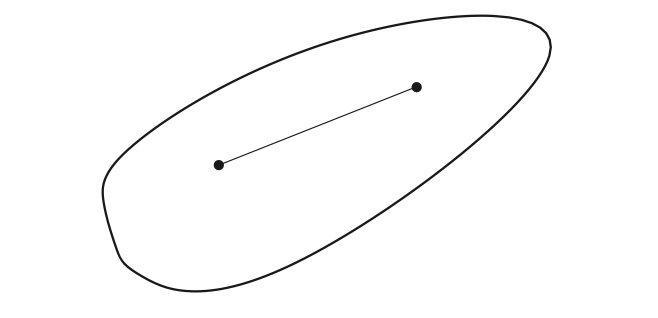
\includegraphics[width=0.6\textwidth]{Images/Fundamental/ConvexSet.png}
    %     \\[1ex] % Adds some space between the image and the caption
    %     \textbf{(a) Convex Set}
    %     \label{fig:convex}
    % \end{minipage}
    % \begin{minipage}[t]{0.48\textwidth}
    %     \centering
    %     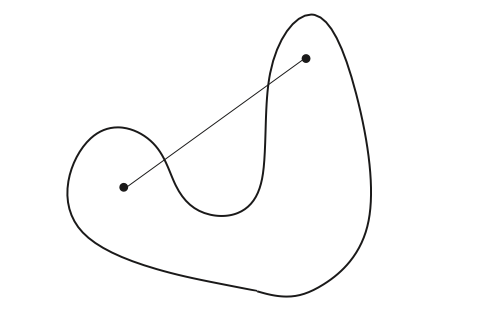
\includegraphics[width=0.6\textwidth]{Images/Fundamental/NonConvexSet.png}
    %     \\[1ex] % Adds some space between the image and the caption
    %     \textbf{(b) Non-Convex Set}
    %     \label{fig:nonconvex}
    % \end{minipage}
\end{theo}

\begin{theo}[Convex function]{ConvexFunction}
    A function $f: \Omega \rightarrow \mathbb{R}$ is convex if 
    \begin{equation*}
        \forall x,y \in \Omega, \ \forall \lambda \in [0,1]: \ f(x + \lambda(y - x)) \leq f(x) + \lambda(f(y) - f(x)).
    \end{equation*}
    or if ``all secants (i\@.e\@. a line segment between two points on the graph) are above graph''. This definition is equivalent to saying that the Epigraph of $f$, i\@.e\@. the set $\{(x,s) \in \mathbb{R}^n \times \R \ | \ x \in \Omega, \ s \geq f(x) \}$, is a convex set.
    \vspace*{-0.1cm}
\end{theo}

\begin{theo}[Convex optimization problem]{ConvexOptimization}
    An optimization problem with convex feasible set $\Omega$ and convex objective function $f: \ \Omega \rightarrow \R$ is called a convex optimization problem. 
\end{theo}

\newpage

\begin{theo}[Globality of local minima of convex optimization problem]{LocalImpliesGlobal}
    For a convex optimization problem, a local minimum is also a global one.
\end{theo}

\begin{prf}[Globality of local minima of convex optimization problem]{prfLocalImpliesGlobal}
    Regard a local minimum $x^*$ of the convex optimization problem 
    \begin{mini*}|l|
        {x \in \mathbb{R}^n}{f(x)}
        {}{}
        \addConstraint{x \in \Omega}.
    \end{mini*}
    We will show that for any point $y \in \Omega$ holds $f(y) \geq f(x^*)$, i\@.e\@. $x^*$ is a global minimum. \\

    \vspace*{0.4cm}

    \begin{minipage}{0.78\textwidth}
        First we choose, using local optimality, a neighborhood $\mathcal{N}$ of $x^*$ such that for all $\tilde{x} \in \Omega \cap \mathcal{N}$ holds $f(\tilde{x}) \geq f(x^*)$. Second, we regard the connecting line between $x^*$ and $y$. This line is completely contained in $\Omega$ due to the convexity of $\Omega$. Now we choose a point $\tilde{x}$ on this line such that it is in the neighborhood, but not equal to $x^*$, i\@.e\@. $\tilde{x} = x^* + \lambda(y - x^*)$ for some $\lambda \in (0,1)$, and $\tilde{x} \in \Omega \cap \mathcal{N}$. Due to local optimality, we have $f(\tilde{x}) \geq f(x^*)$, and due to convexity we have
        \begin{equation*}
            f(\tilde{x}) = f(x^* + \lambda(y - x^*)) \leq f(x^*) + \lambda(f(y) - f(x^*)).
        \end{equation*}
    \end{minipage}
    \begin{minipage}{0.2\textwidth}
        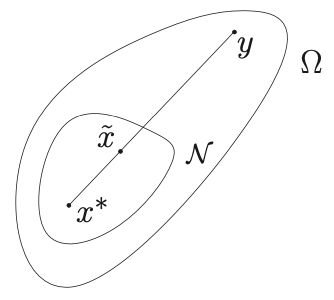
\includegraphics[scale = 0.6]{Images/Fundamental/ProofGlobalityLocal.png}
    \end{minipage}
    \vspace*{0.4cm}

    It follows that $\lambda(f(y) - f(x^*)) \geq 0$, and since $\lambda \in (0,1)$, we have $f(y) \geq f(x^*)$, as desired. 
\end{prf}

\begin{theo}[Unconstrained optimization problem]{UnconstrainedOptimization}
    An optimization problem with no constraints, i\@.e\@. $g(x) = 0$ and $h(x) \geq 0$ are empty, is called an unconstrained optimization problem. 
\end{theo}

\begin{ex}[Nonlinear Programming (NLP)]{NLP}
    Nonlinear Programming Problems are poblems of the following form:
    \begin{mini*}|l|
        {x \in \mathbb{R}^n}{f(x)}
        {}{}
        \addConstraint{g(x) = 0}
        \addConstraint{h(x) \geq 0},
    \end{mini*}
    where $f: \ \R^n \rightarrow \R$, $g: \ \R^n \rightarrow \R^p$, and $h: \ \R^n \rightarrow \R^q$, are assumed to be continuously differentiable at least once.
\end{ex}

\begin{ex}[Linear Programming (LP)]{LP}
    When the functions $f$, $g$, $h$ are affine (i\@.e\@., they can be expressed in the form $f(x) = a^T x + b$ for some vector $a$ and scalar $b$) in the general formulation (see Theorem~\ref{NLP}), the general NLP gets something easier to solve, namely a Linear Program (LP), which can be written as follows:
    \begin{mini*}|l|
        {x \in \mathbb{R}^n}{c^T x}
        {}{}
        \addConstraint{Ax-b = 0}
        \addConstraint{Cx - d \geq 0},
    \end{mini*}
    where $c \in \R^n$, $A \in \R^{p \times n}$, $b \in \R^p$, $C \in \R^{q \times n}$, and $d \in \R^q$.
\end{ex}

\begin{ex}[Quadratic Programming (QP)]{QP}
    When the functions $g$, $h$ are affine (as for an LP in Theorem~\ref{LP}), and the objective function $f$ is a linear-quadratic function, the NLP becomes a Quadratic Program (QP), which can be written as follows:
    \begin{mini*}|l|
        {x \in \mathbb{R}^n}{c^T x + \frac{1}{2}x^T Bx}
        {}{}
        \addConstraint{Ax-b = 0}
        \addConstraint{Cx - d \geq 0},
    \end{mini*}
    where, in addition to the LP parameters, $B \in \R^{n \times n}$ is the Hessian matrix. Specifically, for the objective function $f(x) = c^T x + \frac{1}{2}x^T B x$, the Hessian is given by:
    \begin{equation*}
        \nabla^2 f(x) = B.
    \end{equation*}
    \vspace*{-0.7cm}
\end{ex}

\begin{theo}[Convex QP]{ConvexQP}
    If the Hessian matrix $B$ is positive semi-definite (i\@.e\@. if $\forall z \in \mathbb{R}^n \setminus \{0\}: z^T Bz \geq 0$) we call the QP a convex QP\@. Convex QPs are tremendously easier to solve globally than “non-convex QPs” (i\@.e\@., where the Hessian B is not positive semi-definite), which might have different local minima (i\@.e\@. have a non-convex solution set).
\end{theo}

\begin{theo}[Strictly convex QP]{StrictlyConvexQP}
    If the Hessian matrix $B$ is positive definite (i\@.e\@. if $\forall z \in \mathbb{R}^n \setminus \{0\}: z^T Bz > 0$) we call the QP a strictly convex QP\@. Strictly convex QPs are a subset of convex QPs (see Theorem~\ref{ConvexQP}).
\end{theo}

\newpage

\begin{ex}[Mixed-Integer Programming (MIP)]{MIP}
    A mixed-integer programming problem or mixed-integer program (MIP) is a problem with both real and integer decision variables. A MIP can be formulated as follows:

    \begin{minipage}{0.64\textwidth}
        \begin{mini*}|l|
            {\substack{x \in \mathbb{R}^n \\ z \in \mathbb{Z}^m}}{f(x, z)}   
            {}{}
            \addConstraint{g(x, z) = 0}
            \addConstraint{h(x, z) \geq 0},
        \end{mini*}
        where \( x \in \mathbb{R}^n \) are the continuous variables, and \( z \in \mathbb{Z}^m \) are the integer variables.
    \end{minipage}
    \begin{minipage}{0.36\textwidth}
        \begin{center}
            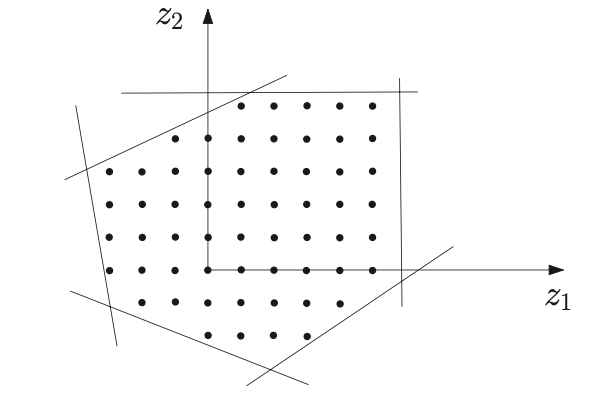
\includegraphics[scale = 0.5]{Images/Fundamental/MIP.png}
        \end{center}
    \end{minipage}
\end{ex}

